% This is samplepaper.tex, a sample chapter demonstrating the
% LLNCS macro package for Springer Computer Science proceedings;
% Version 2.20 of 2017/10/04
%
\documentclass[runningheads]{llncs}
%
\usepackage{graphicx}
\usepackage{url}
\usepackage{mathtools}

% Used for displaying a sample figure. If possible, figure files should
% be included in EPS format.
%
% If you use the hyperref package, please uncomment the following line
% to display URLs in blue roman font according to Springer's eBook style:
% \renewcommand\UrlFont{\color{blue}\rmfamily}

\begin{document}
%
\title{Clinical Pneumonia Classification Based on CT Attenuation via Multi-Source Information Fusion}
%
%\titlerunning{Abbreviated paper title}
% If the paper title is too long for the running head, you can set
% an abbreviated paper title here
%
\author{Qiuli Wang\inst{1}\and
Zhihuan Li\inst{1} \and
Sheng Huang\inst{1} \and
Chen Liu\inst{2}\and
Xiaohong Zhang\inst{1}\and
Dan Yang \inst{1}
}
%
\authorrunning{Q.Wang et al.}
\titlerunning{Pneumonia Classification}
% First names are abbreviated in the running head.
% If there are more than two authors, 'et al.' is used.
%
\institute{School of Big Data \& Software Engineering, Chongqing University, 400000, Chongqing , China \\ \email{\{wangqiuli, lizhihuan, huangsheng, xhongzh, dyang\}@cqu.edu.cn}\\\and
Radiology Department, The First Affiliated Hospital of Army Medical University,400000, Chongqing, China \\
\email{cqliuchen@foxmail.com}
}
%
\maketitle              % typeset the header of the contribution
%
\begin{abstract}
Existing CAD(Computer Aided Detection) systems for pneumonia diagnosis are basically designed for X-ray image. But in clinical application, CT(Computed Tomography) has become the most common technology for diagnosing pneumonia. Compared with X-ray image, CT scans have a more clear view of patients' bodies, contain more information, have bigger data size and are more complicated. As a result, applying deep learning directly to raw CT scans requires much resource of computing.
Inspired by the diagnosis precess of radiologists, we treat reading CT scans as playing short videos. So we transform the problems of classifying CT scans into the problems of classifying videos.
In this study, we combine  CNN(Convolutional Neural Network) with LSTM(Long Short Term Memory).
We use CNN to extract features of each scan of CT and get a sequence of features, and feet them to LSTM to predict pneumonia.  In order to extract more information from CT, we extract information from three different attention from CT volume and use them as three channel.
We use a auxiliary loss to speed up the training process. 
Our model achieve 0.925 in accuracy, and have a very balance performance in accuracy, sensitivity and specificity.


\keywords{Long Short Term Memory(LSTM) \and Pneumonia Diagnosis \and Convolutional Neural Network \and Computed tomography (CT) \and Computer-aided detection and diagnosis (CAD) \and Multi-Source Information}
\end{abstract}

\section{Introduction}
Chest X-rays used to be the best available method for diagnosing pneumonia, playing a crucial role in clinical care\cite{Franquet2001Imaging} and epidemiological studies\cite{Thomas2005Standardized}. However, with the development of economic, CT(Computed Tomography) has become the most common technology for diagnosing pneumonia in China. According the radiologists, a radiologist of the major hospital need to read hundreds scans of CT every day. Thus, developing a fast, robust and accurate CAD system to perform automated diagnosis of pneumonia is meaningful and important. 

There have been lots of models designed for diagnosing thoracic diseases.
Hoo-Chang Shin \cite{Shin2016Learning} combined CNN and LSTM,  made the model have the ability of 'reading' chest X-Rays. This model used CNN to extract features from chest X-Ray and used LSTM to generated MeSH\cite{timmurphy.org} terms for image. In 2017, Xiaosong Wang et al.\cite{Wang2017ChestX} provided hospital-scale chest X-ray database ChestX-ray8 which contains eight common thoracic diseases. This database allow researchers use deeper neural network to analyze medical images. Based on this dataset, Pranav Rajpurkar, Andrew Y. Ng et al. \cite{Rajpurkar2017CheXNet} developed CheXnet with 121-layer. This model achieved an F1 score of 0.435, higher than human radiologists. Xiaosong Wang et al.\cite{Wang2018TieNet} proposed TieNet, which can classify the chest X-Rays into different diseases and generate the report at the same time. In TieNet, CNN was used capture features of chest X-Rays, RNN was used to generate report, and attention mechanism was used to help RNN to focus on different parts of images with the generation of reports. 

Studies above have something in common. First of all, they were designed for chest X-Rays, which means these methods can only handle 2D images. Even if models can achieve good results in every indication, these models still cannot handle CT(Computed Tomography) scans, which is commonly used in clinical practice. Compared with  X-Rays, CT scans contain much more complex information.  Each slice in CT scans is a 2D image of human body, using these 2-D slices can reconstruct 3-D structure of human bodies. Moreover, CT scans  have a more clear view of patients' bodies, since ribs and clavicles won't cast shadows in front of chest. As a result, CT scans have a much larger data size. One series of chest CT contains hundreds of slices and each slice has a size of $512 \times 512$.  Extensive studies show that 3D CNN is  the best choice for keeping 3D spatial information in the CT scans \cite{Yorozu1987Electron}. However, 3-D CNN cannot be applied to raw CT data directly since it will bring a heavy burden to the server. 

Second, for models designed for diseases diagnosing like CheXnet, few of them combine image information with other information about patients like gender, age. For models like TieNet, they combine image information with descriptions from radiologists, but descriptions from radiologists still contain no information for patients cause descriptions is only related to images, this descriptions only help models understand image without knowing anything about patients themselves, which is contrary to che clinical diagnosis process. Patients' complaints is a very useful information when doctors are diagnosing, because complaints is patients direct feeling about their physical condition. However, as far as we know, few studies use this information to improve the performance of CAD systems.

In general, there two major problems of existing CAD systems: 1, they cannot handle CT scans and 3-D information, and this problem has become a practical limitation; 2, they only analysis images or information about images, but seldom consider information about patients.

In this study, we treat slices of CT scans as video frames, and transform the problems of classifying CT scans into the problems of classifying videos. We use RCNN(Recurrent Convolutional Neural Network) to extract features from slices of CT scans. Moreover, we embed patients' complaints into word vector
\cite{mikolov2013efficient}\cite{mikolov2013distributed} and use LSTM(Long Short Term Memory) to extract features, and concatenate it with features of images, alone with information about patients' age and gender. Finally, we propose a MSID(Multi-Source Information Diagnosis) model.
We compare VGG\cite{simonyan2015very}, ResNet\cite{he2016deep} and Inception-V3 \cite{szegedy2016rethinking} and choose ResNet50 to capture visual features. Follow the study in \cite{Donahue2015Long}, we use LSTM(Long Short Term Memory)\cite{hochreiter1997long} as RNN cells. 
Studies in \cite{gao2018holistic} and \cite{Shin2017Three} extract HU values from CT volume and transform them into three different range:normal[-1400, 200HU], high attenuation [-160, 240HU], low attenuation [-1400, -950HU]. We adjust normal[-1400, 200HU] to [-1000, 400HU] according to the instruction from LUNA16\cite{Aaa2016Validation}, and make these three one-channel images with different range of HU values into one three-channel image and feed it into model. We use raw data from a major hospital and analysis 1002 cases. Our model achieve 0.945 in accuracy and 0.9358 in sensitivity.

\section{Data}
\label{data}
\subsection{CT Image Data and Multi-Source Information}
\label{ctimagedata}
Because the shortage of public CT dataset for pneumonia, we use raw data from a major hospital. We get 1036 cases of CT(842  patients with pneumonia, 464 people are healthy) from hospital PACS(Picture Archiving and Communication Systems). We open a CT scan with RadiAnt DICOM Viewer$\footnote[1]{www.radiantviewer.com}$, as shown in Fig~\ref{reader}, raw data from hospital may have more than one series of images(yellow rectangle), each series may have different data type or different image windows, doctors or radiologists may read details of images from main area of reader(red rectangle), but for models who needs to learn information from data, it has no image viewer for images. It means raw data cannot be used directly for deep learning models, so we adjust the data appropriately.

First of all, we eliminate these cases which  start scanning from middle of the chest. Then we pick up the best series from the whole cases according to the following requirements:

1. We use the series with the specific `Convolution Kernel', which can make the CT more suitable for observing the lungs or chest, for example, in Fig~\ref{Bs}, image under B70s has clearer view of lungs, image under B41s has clearer view of heart. More specifically, we choose `B31f', `I31f 3', `B70f', `B80f', `B70s', since  radiologists use these `Convolution Kernels'  frequently to observe the lungs and chest. Number of different `Convolution Kernel' is shown in Fig~\ref{NumberofDifferentConvolutionKernel}. However, different `Convolution Kernels' will not affect images we analysis in the end, because all images will be calculated and transformed into HU unit, which will be discussed in section~\ref{preprocessing}.

2. We calculate `Slice Thickness' of each series, and keep series with the smallest `Slice Thickness', since small thickness may keep more detailed information of body structure. 

3. If there were more than one series meet the last two requirements, we will keep the series with the largest number of scans, which can have a larger span.

As a result, we keep 552 cases with pneumonia and 450 cases of healthy people (1002 cases total).
We split dataset in training/validation/testing as 60\% /20\% /20\% and make them identically distributed in three parts of datasets, so we have 6002 cases in training set, 200 cases in validation set, 200 cases in test set.
Number of healthy and pneumonic cases in different slice-thickness is shown in Table~\ref{distributionofhealthyandpneumonic}.

Each CT scan has a case file. In case files, we can get patients basic information: patient ID, gender, age. Moreover, each case file contains patient complaint. Patient complaints are descriptions from patients which describe their own feeling about their condition, which is very important in clinical practice. In this study, we will use gender, age as additional attributes, and use LSTM extract attributes from patients' complaints, and combine them with attributes from CT scans.

\begin{figure}[t]
\centerline{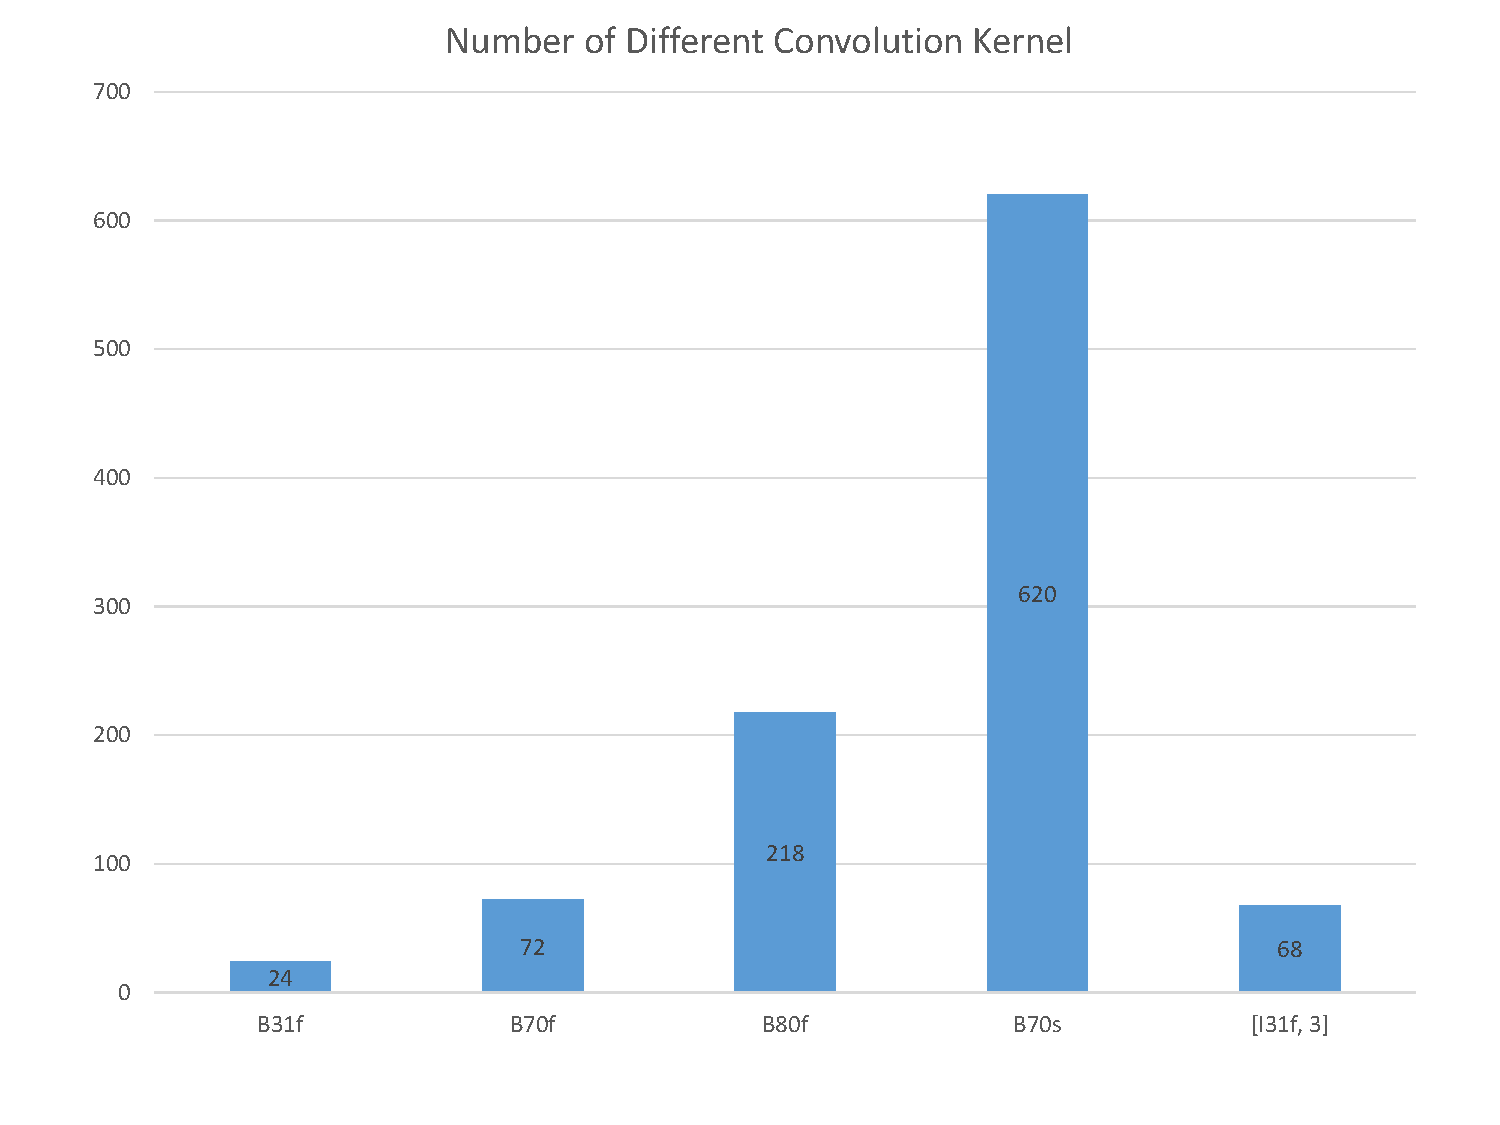
\includegraphics[width=100mm]{NumberofDifferentConvolutionKernel.pdf}}
\vspace{-0cm}
\caption{Number of Different Convolution Kernel}
\vspace{-0cm}
\label{NumberofDifferentConvolutionKernel}
\end{figure}

\begin{figure}[t]
    \centerline{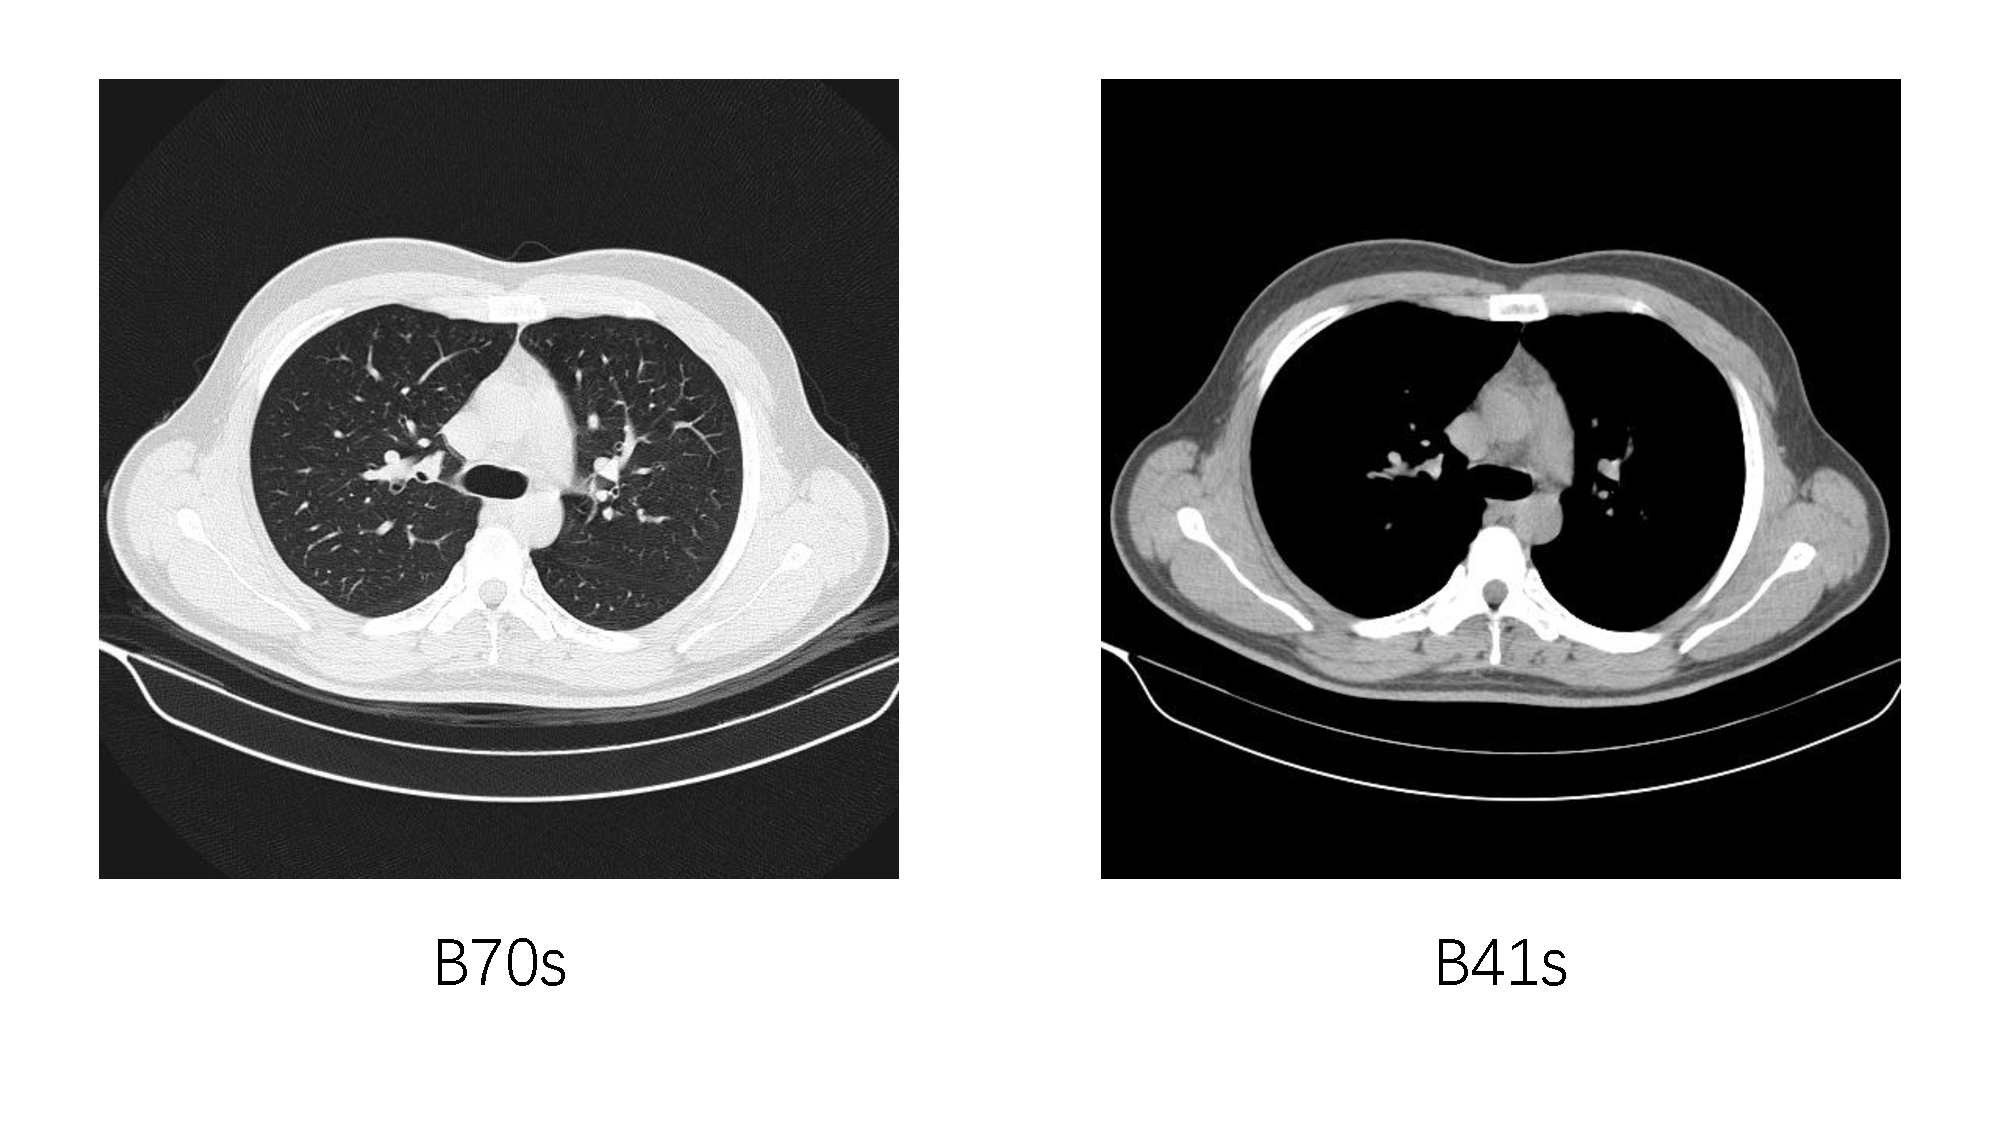
\includegraphics[width=100mm]{Bs.pdf}}
    \vspace{-0cm}
    \caption{Scans with Different Convolutional Kernel}
    \vspace{-0cm}
    \label{Bs}
    \end{figure}

\begin{figure}[t]
    \centerline{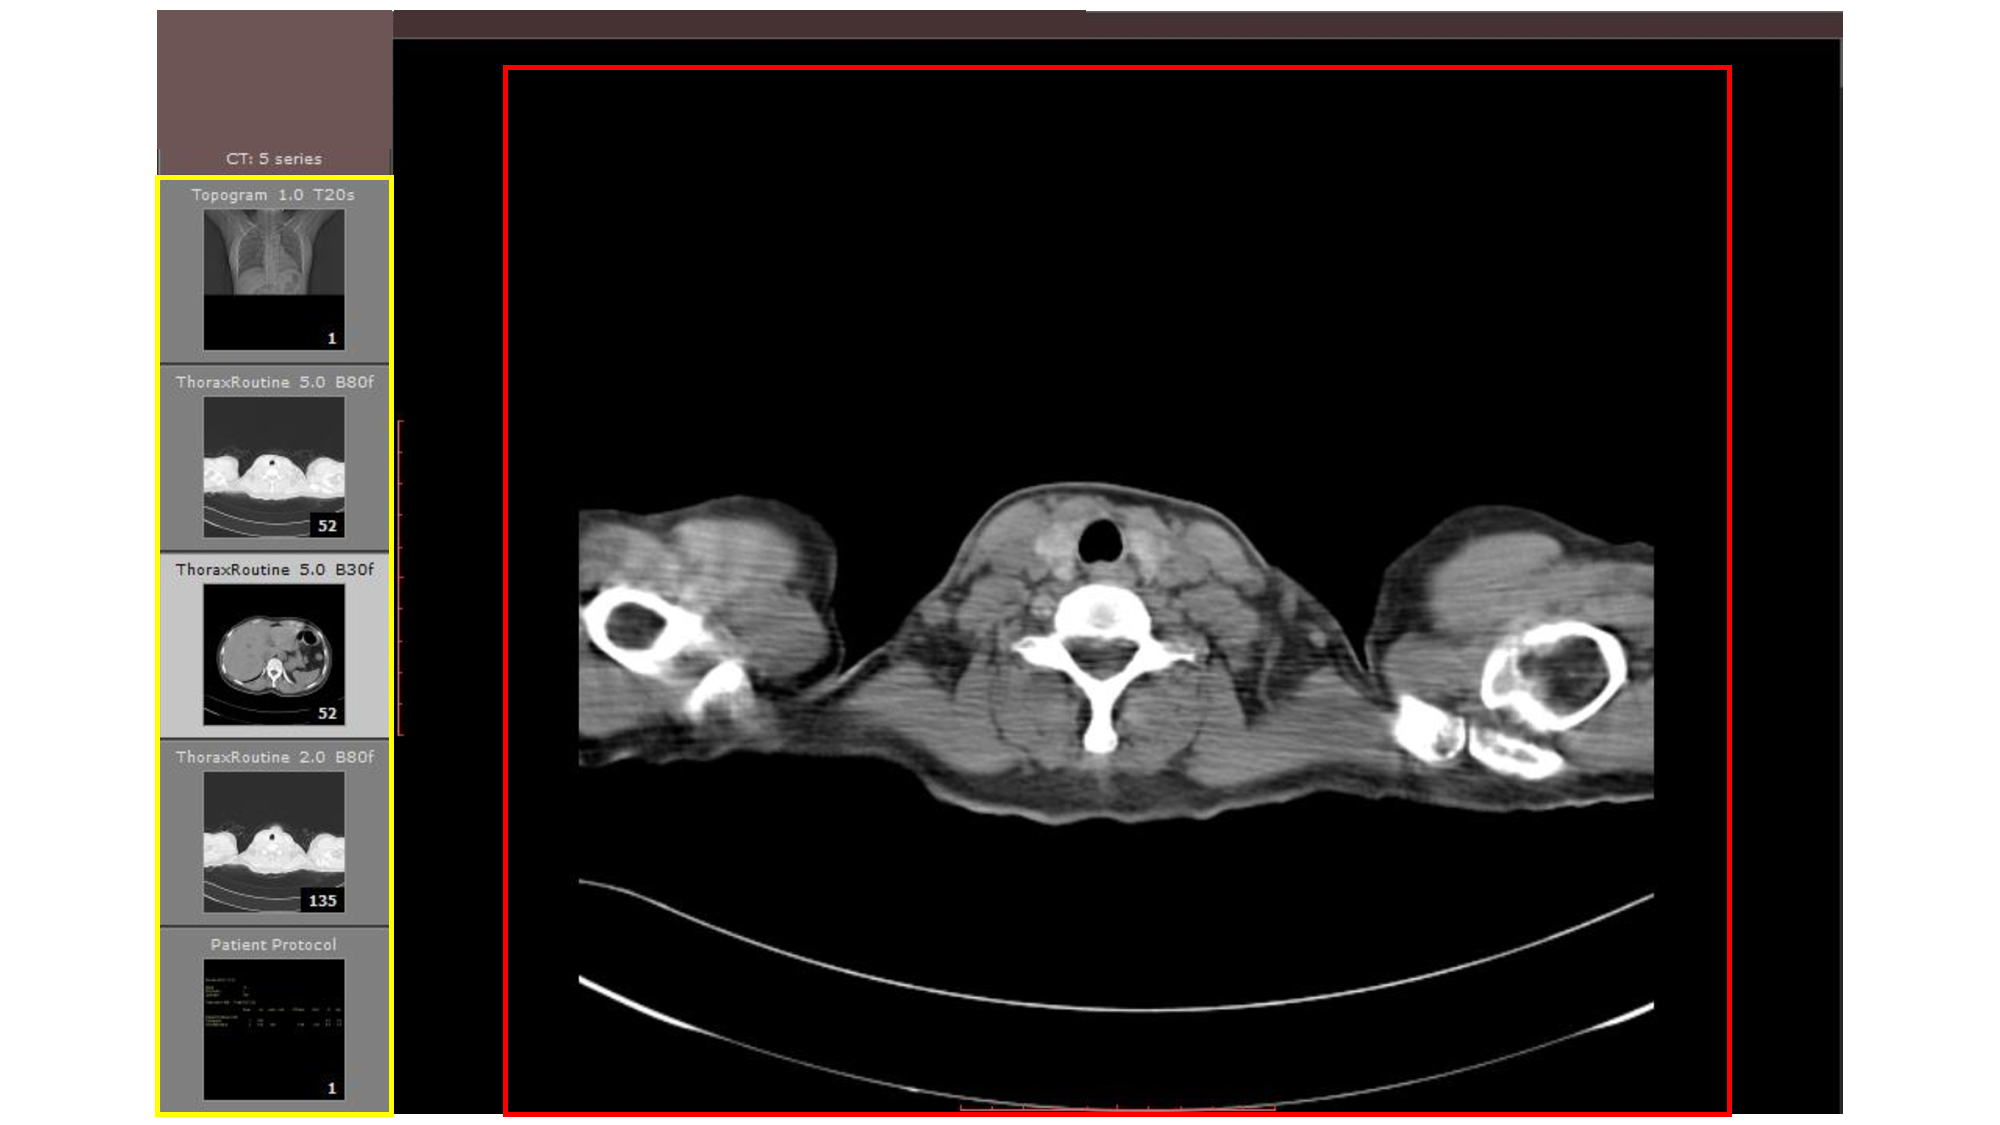
\includegraphics[width=150mm]{reader.pdf}}
    \vspace{-0cm}
    \caption{Structure of Raw Data from Hospital}
    \vspace{-0cm}
    \label{reader}
    \end{figure}

\begin{table}[htb]
\vspace{-0cm}
\caption{Number of Healthy and Pneumonic Cases in Different Slice-Thickness}
\vspace{-0cm}
\begin{center}
\begin{tabular}{|c|c|c|}
\hline
\textbf{\textit{Slice-Thickness}}& \textbf{\textit{Healthy}}& \textbf{\textit{Pneumonic}}  \\
\hline
1 mm & 0 & 24 \\
1.5 mm  & 1 & 7\\
2 mm & 444 & 386  \\
3 mm & 0 & 127  \\
5 mm & 5 & 8  \\
\hline
Total & 450 & 552 \\
\hline
\end{tabular}
\vspace{-0cm}
\label{distributionofhealthyandpneumonic}
\end{center}
\vspace{-0cm}
\end{table}

\subsection{Data Preprocessing}
\label{preprocessing}
\subsubsection{CT Image Data}
\label{ctimagedata}
There are kinds of image windows for CT reader, such as windows for bone, brain, chest, lungs. Images under different image windows will highlight different tissues of bodies.
As mentioned in section\ref{ctimagedata}, there kinds of `Convolution Kernel' within different CT volume. Each kind of `Convolution Kernel' in fact can show specific window for CT images. But it may make data inconsistent. So we transform raw data into HU(Hounsfield Unit) values. The Hounsfield unit named after Sir Godfrey Hounsfield, is a quantitative scale for describing radio-density, its value is also termed CT number. After transformed into HU values, all slices form CT scans will have the same unit of measure, then we ill transform this images into the same HU ranges.

Follow the study in \cite{Shin2017Three}, we use three image windows: normal[-1000, 400HU], high attenuation [-160, 240HU], low attenuation [-1400, -950HU]. In Fig\ref{3channel} we can see that, compared to original CT image, image in `Normal' is brighter, tissues in lungs are clearer and details are enhanced. Image in `High Attenuation' have a clear view of hearts and vessels(in yellow rectangle). `High Attenuation' range also enhance the difference between high density pathological tissues(in white rectangle) and normal tissues. `Low Attenuation' range highlight abnormal voids in lungs(in red rectangle) which is features of severe lung diseases. All images mentioned above are one-channel grey level images, and we finally combine three ranges images into 3-channel images which fits the requirements of CNN models, if we save 3-channel images, we will find out that these images actually are false color images, as shown in Fig~\ref{3channel}. The `Slice Thickness' between each slice is adjusted into 10mm, and each scan will keep 32 slices.
The influence of different range will be discussed int section~\ref{exp}.

\begin{figure}[t]
    \centerline{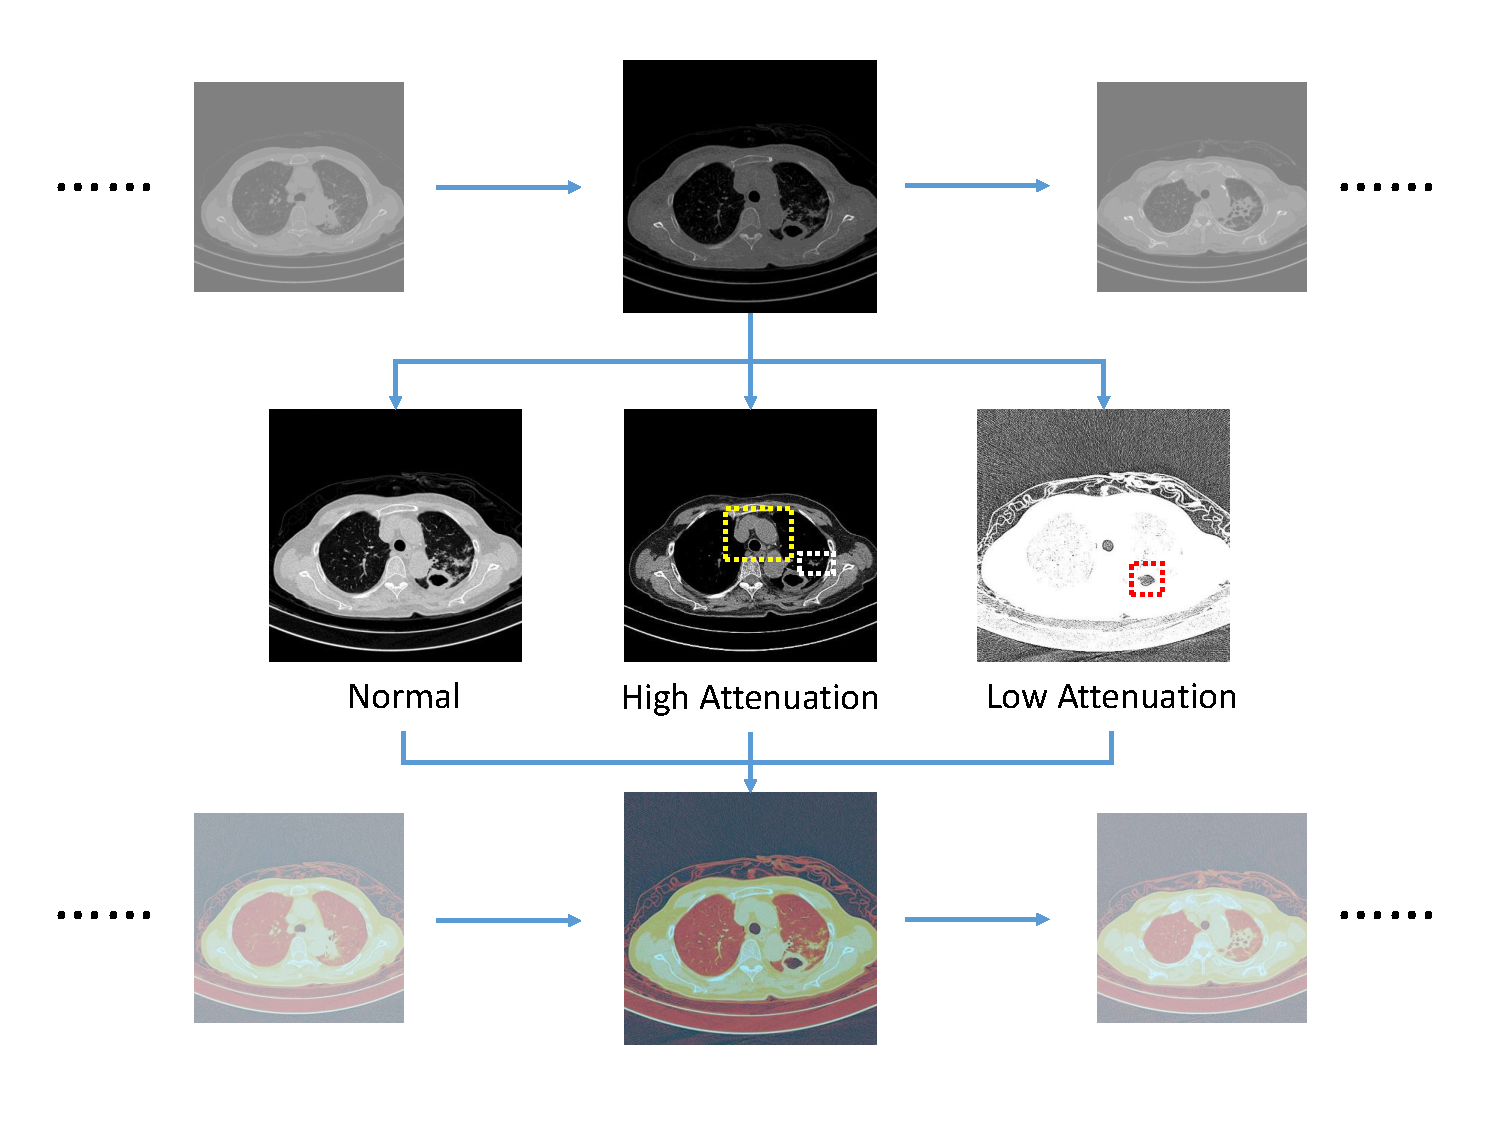
\includegraphics[width=150mm]{3channel.pdf}}
    \vspace{-0cm}
    \caption{Data Pre-precess for CT Scans}
    \vspace{-0cm}
    \label{3channel}
    \end{figure}

\subsubsection{Patient Age, Gender and Complaints}
\label{textdata}
The pre-process of age, gender and complaints is shown in Fig~\ref{textinfo}. For each patient, we have a list of information contains age, gender and complaints. 
For patient age and gender, we transform them into numbers. Gender information will be transformed into a two-dimensional array, [1, 0] represents male, [0, 1] represents female. Age will be calculated according to patient birthday. For example, patient in \ref{textinfo} is an adult male, who was born in 1999-10-29. His gender and age will be transformed to [1, 0] and 20.

For patients' complaints, since we only have Chinese complaints, we have to do Chinese word segmentation. Chinese word segmentation is a very difficult problem so we will take a short cut. We use a mature tools: Jieba text segmentation$\footnote[2]{https://github.com/fxsjy/jieba}$ to segment Chinese sentences into Chinese word sequences so that LSTM can analysis them. Before segmentation, we remove numbers, punctuation marks in order to get a better segmentation results. An example of Chinese word segmentation is shown in green rectangle in Fig~\ref{textinfo}. However, English patient complaints have no need to do segmentation. If you use data from English speaking country, you may skip this step.
After segmentation, we use word2vec to embed word sequences into vectors. We use CBOW(Continuous Bag-of-Words)\cite{mikolov2013efficient} to capture relationship between words. Since our corpus is very small, we set embedding size as 50, and window size as 3. In order to simplify model, we set length of Chinese word sequence to 16 since 16 is the maximum length among all complaint sequences. For those sequences whose length is less than 16, we add `None' to fill up the voids and increase  length to 16. The details of word2vec will not be discussed here. After embedding, each word will be embedded into a vector of 50 dimensions.

Code for data preprocessing will be released very soon.
\begin{figure}[t]
    \centerline{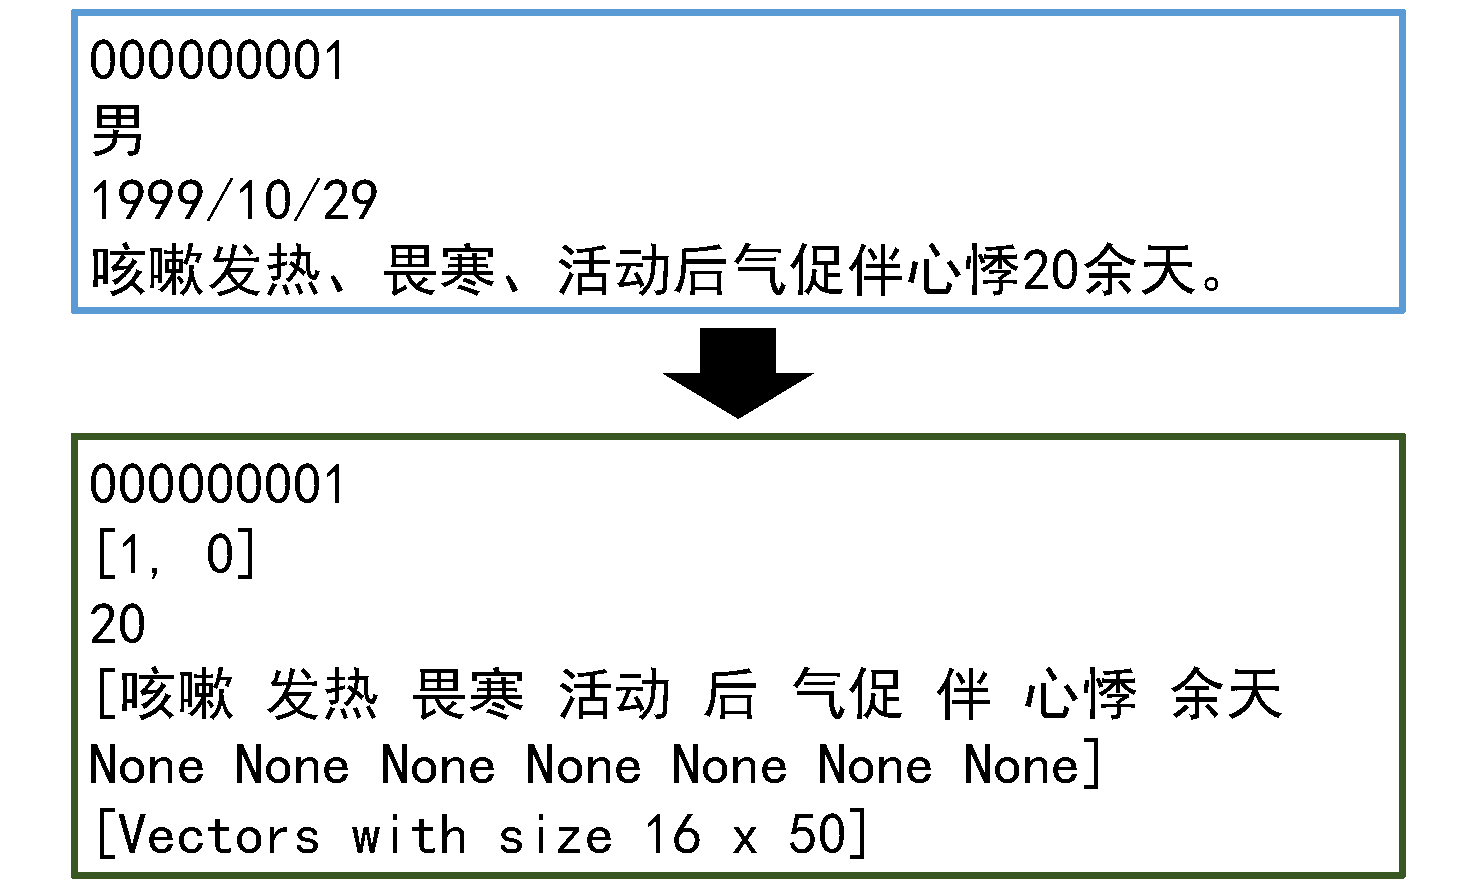
\includegraphics[width=90mm]{textinfo.pdf}}
    \vspace{-0cm}
    \caption{Data Pre-precess for Age, Gender and Complaints}
    \vspace{-0cm}
    \label{textinfo}
    \end{figure}



\section{Method}
\label{method}

\subsection{Recurrent Convolutional Neural Network}
\label{RCNN}
RCNN(Recurrent Convolutional Neural Network) has been proved to be very useful for video caption, description and classification \cite{Donahue2015Long}\cite{Aafaq2019Spatio}, however, only a few work apply RCNN to medical image analysis. Zreik, Majd et al. \cite{Zreik2018A} recently use RCNN for automatic detection and classification of coronary artery plaque, they use CNN extracts features out of $ 25\times25\times25$ voxels cubes, and  use an RNN to processes the entire sequence using gated recurrent units (GRUs). They prove that RCNN is potential for sequence information processing of medical images. 
Follow the study\cite{Donahue2015Long}, we use LSTM as our RNN cells cause LSTM has been demonstrated to be capable of large-scale learning of sequence data. However, few studies have paid attention to different CNN models' performance on medical images, so we try three kinds of classic CNN models: VGG16, ResNet50 and GoogleNet with Inception-V3. Experiments show that ResNet50 has the most stable performance, so that we use ResNet50 as feature extractor of images. Moreover, we wanted to test deeper models like ResNet101, but it will cost more resource of calculation, so we still keep ResNet50.
We test different models with images with different ranges of HU value, which will be discussed in section~\ref{exp}.

We use ResNet50 without fully connected layers as feature extractor. Fig~\ref{resnetall} shows the architecture of ResNet50 blocks. As we all know, block provide shortcut connection between input and outputs of three convolutional layers and allow us to build very deep CNN model.

\begin{figure}[htb]
    \caption{Architecture of ResNet50 Block}
    \centerline{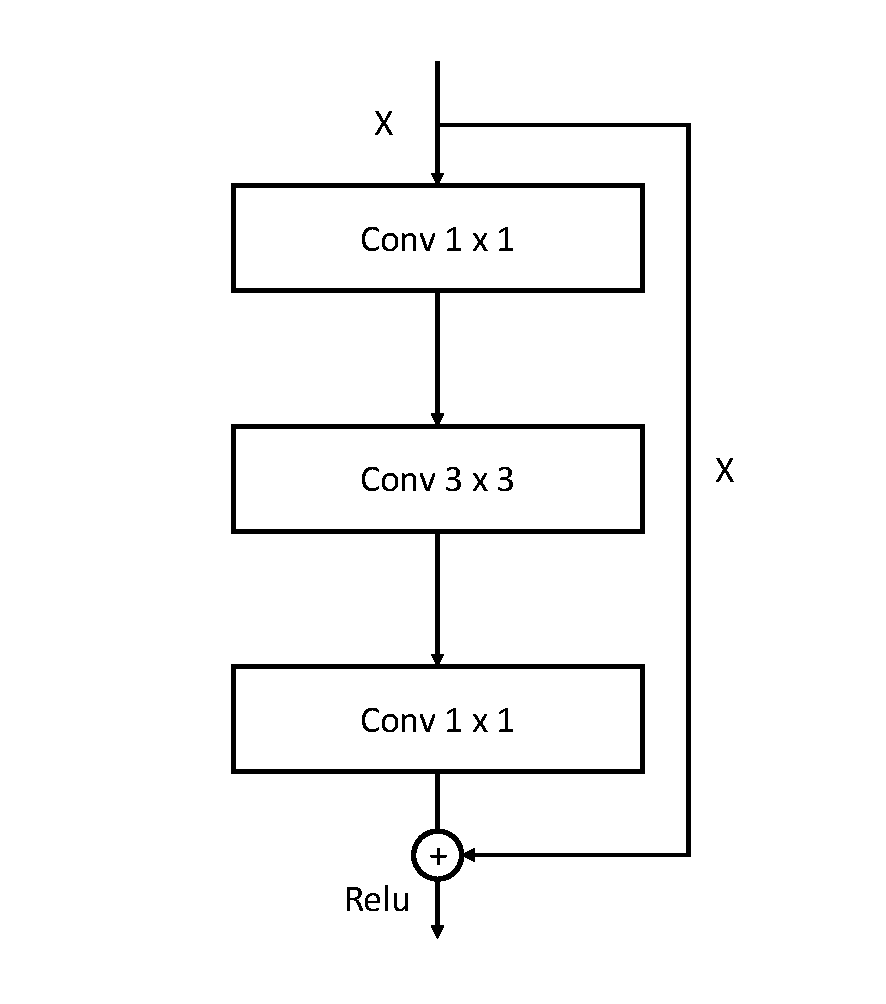
\includegraphics[width=50mm]{resnet.pdf}}
    \vspace{-0cm}
    \vspace{-0cm}
    \label{resnetall}
    \end{figure}

The input size of model is $512 \times 512$, so the outputs of CNN will be $16 \times 16 \times 2048$. If we use fully-connected layer, the length of first fully-connected layer will be $1 \times 524288$, which will make this model very difficult to train. So we use global average pooling proposed in study\cite{lin2014network}, as shown in Fig~\ref{gap}, which is a replacement of fully-connected layers to enable the summing of spatial information of feature maps, and reduce the greatly reduce the number of neurons. 
After global average pooling, feature maps from CNN will be reshaped into a tensor of size $1 \times 2048$, then we use a fully-connected layer to change this tensor into $1 \times 256$, and feed it into a RNN layer with 256 LSTM units. In order to get the best CNN for RCNN, we use output of LSTM to classify CT scans. The experiments show that ResNet50 performs best in these three models, so our RCNN use ResNet50 as its CNN part, and use one layer of LSTM as its RNN part. In fact, LSTM layer plays the role of encoder, it takes the output of last step and encodes image feature sequences into a middle state $hv_t$ as follows:
\begin{equation}
hv_t = LSTM(Fx_t, hv_{t-1}, z_{t-1})
\label{hvt}
\end{equation}
$Fx_t$ is the $t$-th visual features in CT slices, $hv_{t-1}$ is LSTM hidden state of $t-1$ step, $z_{t-1}$ is LSTM output of $t-1$ step. $t$ is the length of slices, in this study, $t$ is equal to 32.

\begin{figure}[htb]
    \centerline{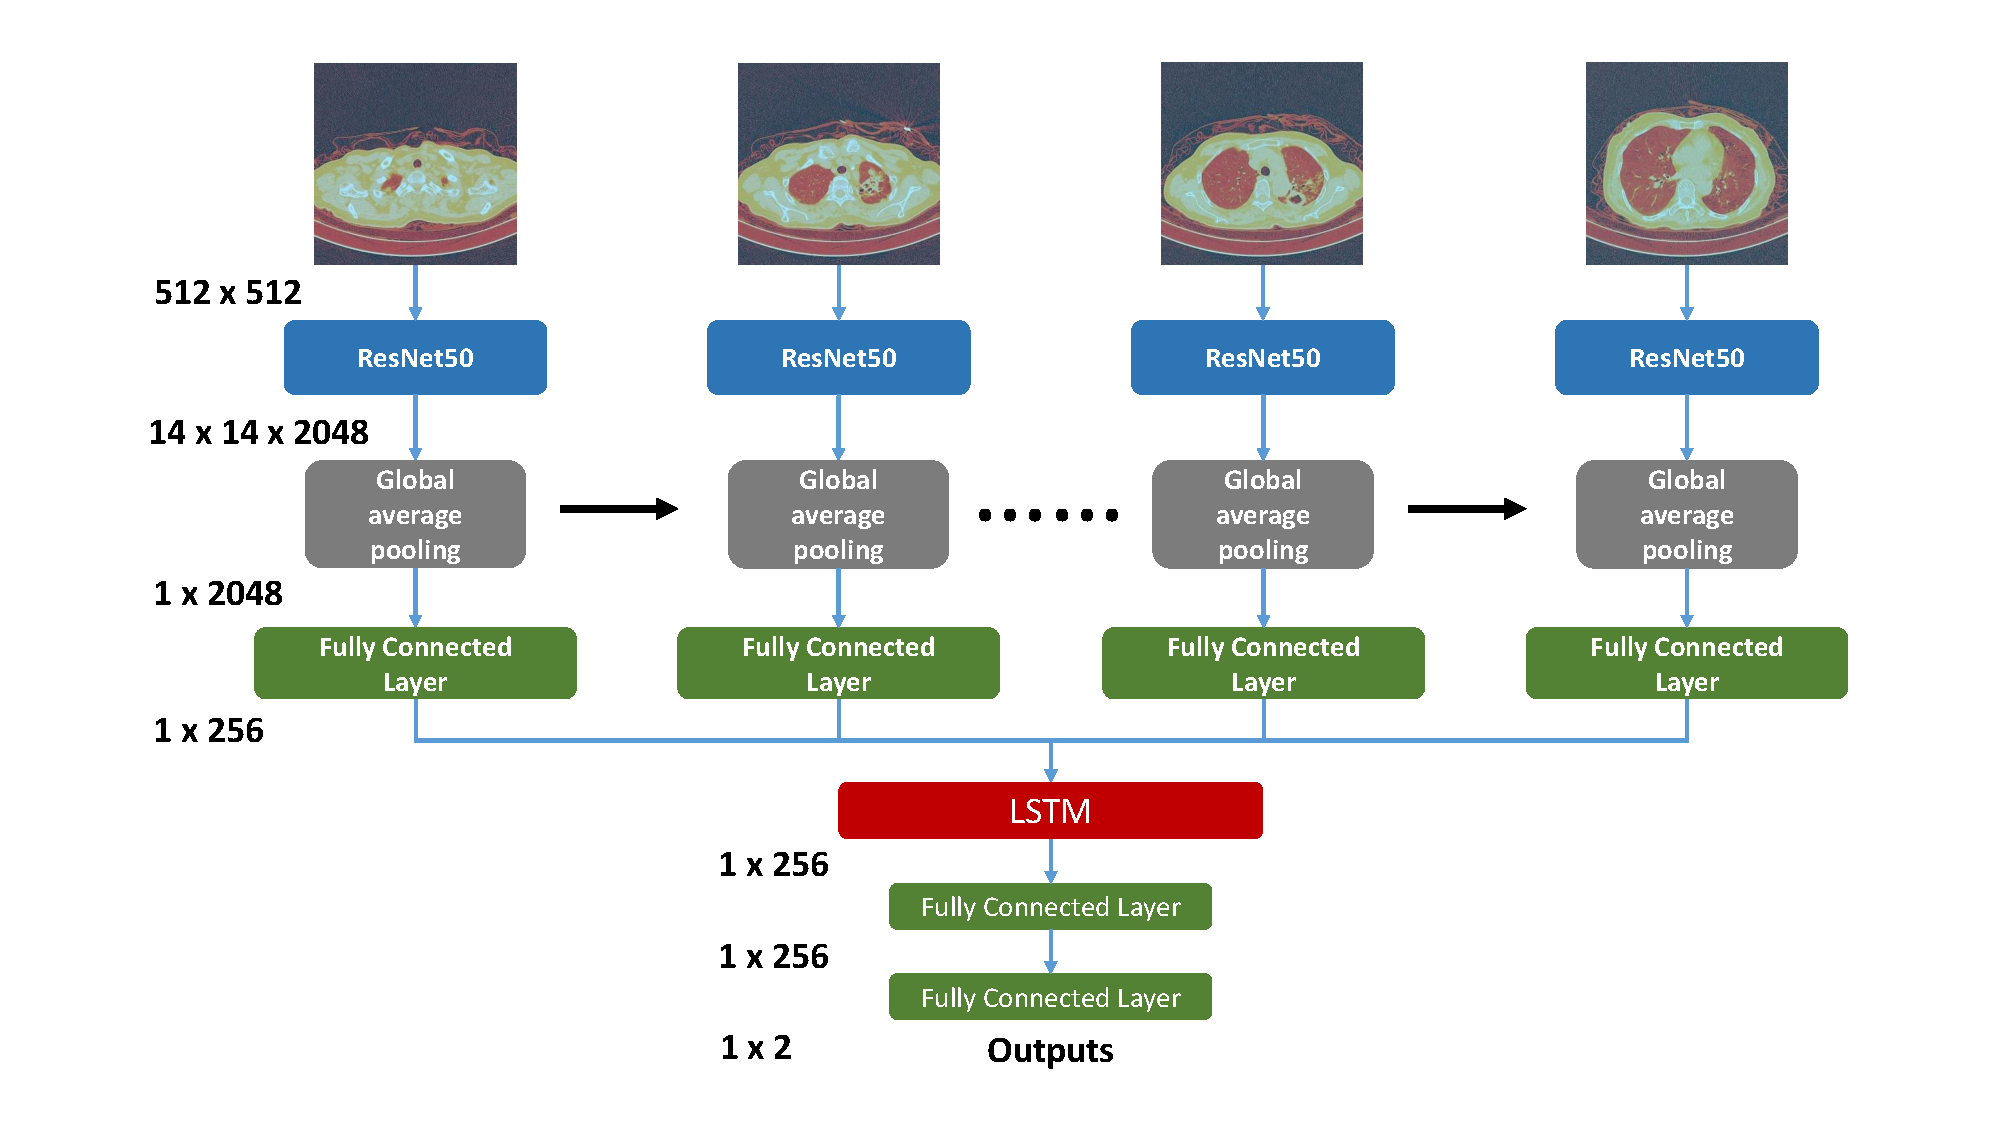
\includegraphics[width=130mm]{onestream.pdf}}
    \vspace{-0cm}
    \caption{Architecture of RCNN}
    \vspace{-0cm}
    \label{onestream}
    \end{figure}

\begin{figure}[htb]
    \centerline{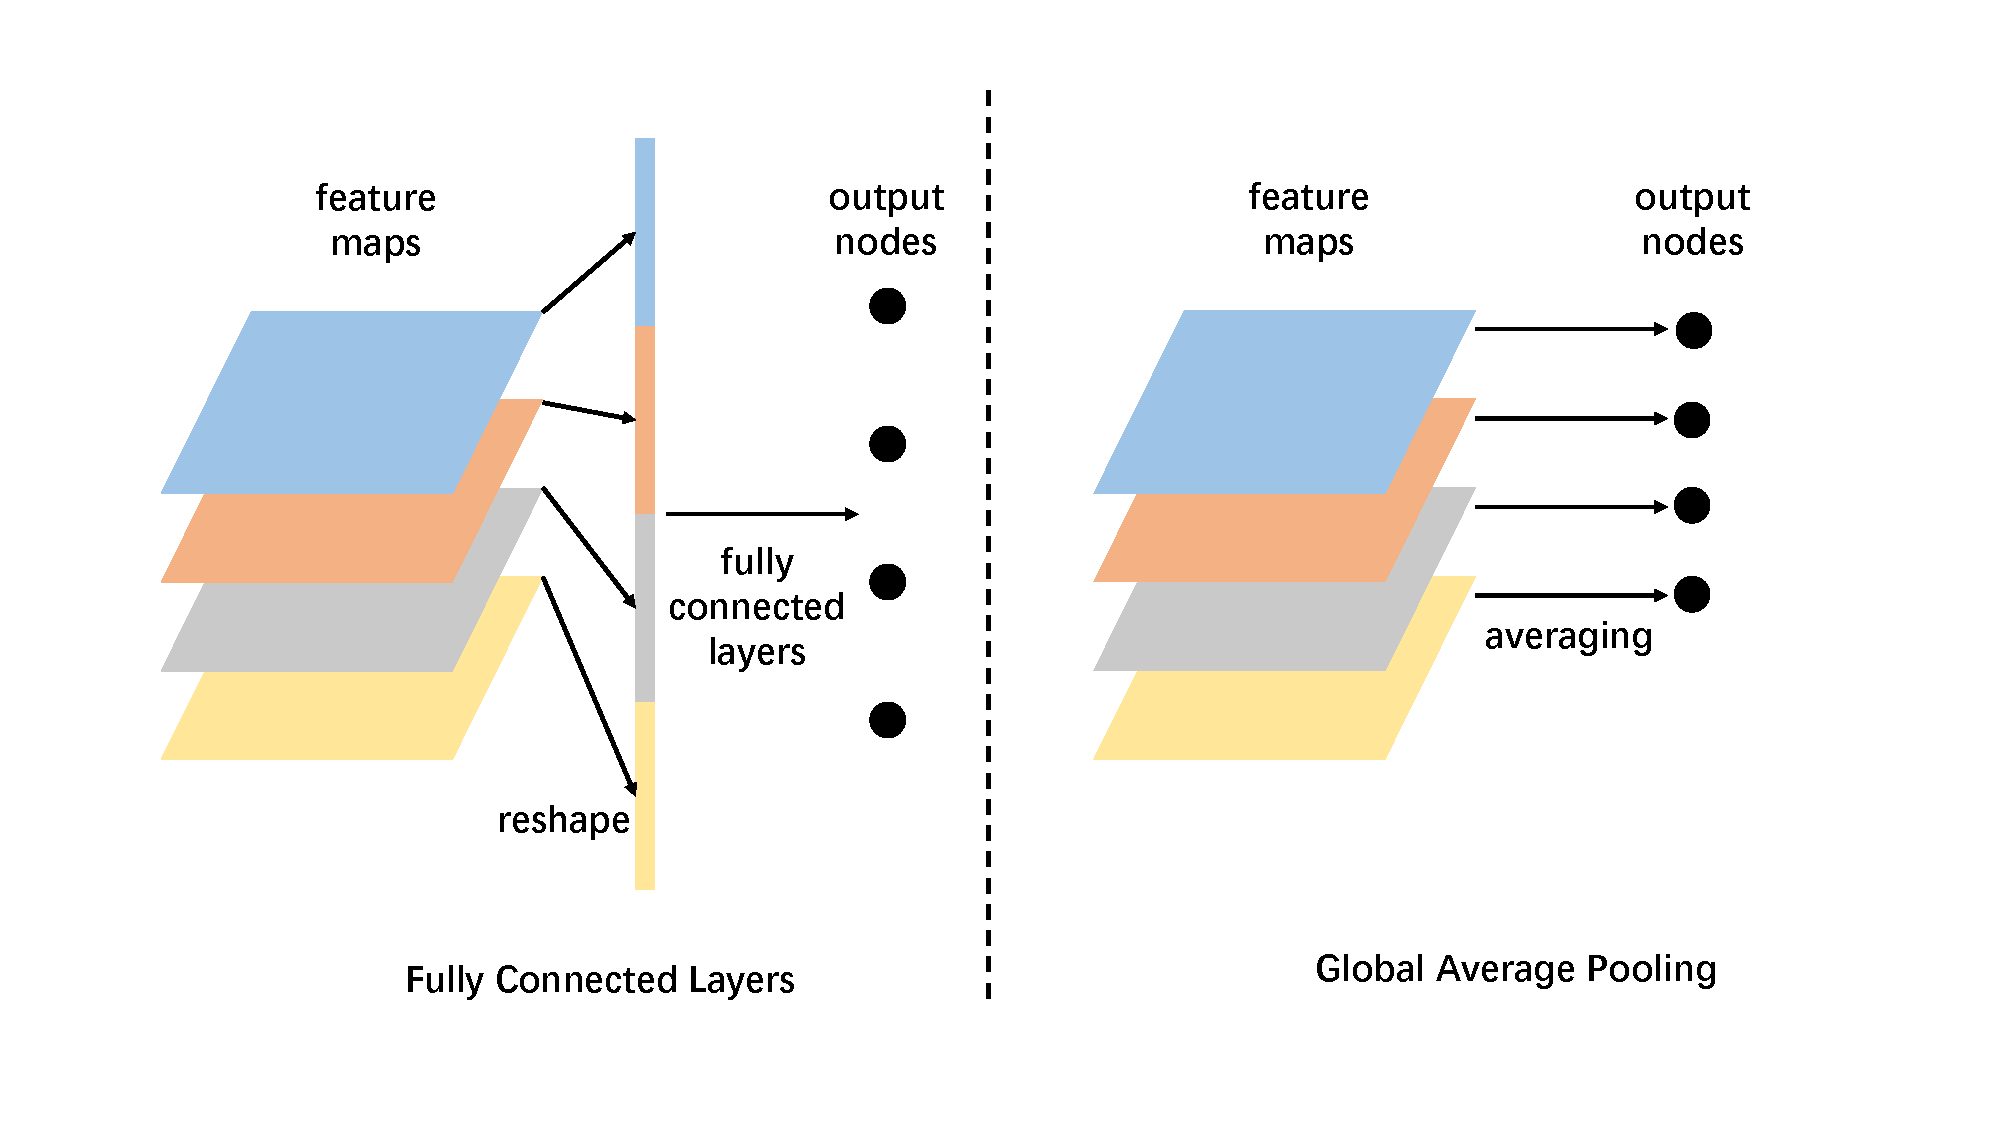
\includegraphics[width=100mm]{gap.pdf}}
    \vspace{-0cm}
    \caption{Difference between Fully Connected Layers and Global Average Pooling}
    \vspace{-0cm}
    \label{gap}
    \end{figure}


\subsection{Multi-Source Information Fusion and MSID}
\label{msid}
Besides CT image information, we also know patients gender, age, and complaints. For gender and age, we use them as additional attributes and set two tensors with size $1 \times 1$ to hold them. For patients' complaints, as mentioned in section~\ref{preprocessing}, we will use Jieba Chinese word segmentation tool to segment Chinese sentences into word sequences. As mentioned in section~\ref{textdata}, we set length of Chinese word sequence to 16. Then we transform sequences of words into sequences of vectors using word2vec, which is commonly used in nature language process, since it can capture the relations between words, the width of vectors is set to 50, so does the number of LSTM units. This LSTM is the second encoder to encode complaint. It is calculated in the same way as equation~\ref{hvt}:
\begin{equation}
    hc_{ct} = LSTM(Cx_{ct}, hc_{ct-1}, z_{ct-1})
    \label{hct}
\end{equation}
$Cx_ct$ is word embedding matrix of the $ct$-th word in complaint, $hc_{ct-1}$ is LSTM hidden state of $ct-1$ step. $ct$ is the length of complaint, which is 16. 
Follow the study \cite{Zreik2018A}, we use cross-entropy as classification loss function. After getting $hv_t$, $hc_{ct}$, we can calculate the prediction and loss as follows:
\begin{align*}\label{classifyandloss1}
    loss1 &= \sum_i{y_i log(\Delta_i)}, \\
    \Delta &= Softmax(F(hv_t \bigotimes hc_{ct} \bigotimes A \bigotimes G))
\end{align*}

where $y_i$ are vectors for the labels of patients, $\Delta$ is prediction after Softmax, $\bigotimes$ is the concatenation operation, $F$ is a function to fuse $hv_t$, $hc_{ct}$, $A$ and $G$, in this study, we simply use two fully-connected layers to fit the function. $A$ is patient age, $G$ is patient gender.

Since LTSM need to analysis 32 feature sequence, we assume that the gradients propagate to CNN will be very small, so that CNN will not be trained properly. Invoked by study in \cite{szegedy2016rethinking}, we use a auxiliary loss to enhance signal of gradient for CNN.
The auxiliary loss is defined as follow: 
\begin{align*}
Loss &=  (1 - \omega) \times loss1 +  \omega \times loss2 \\
loss2 &= \sum_i{y_i log(\Delta^c_i)}
\end{align*}
where $\omega$ is a parameter that within the interval (0, 1).$loss2$ is classification cross-entropy loss from CNN, $\Delta^c_i$ is Softmax prediction of CNN. $\omega$ can adjust the weight of two loss at different training phase.
We expect that at the beginning of training, CNN get stronger gradient and learning to capture features from CT images more quickly. After parameters of CNN get stable, $ loss1$ tends to get small and keep updating parameters of LSTM. We output weights of two losses during training MSID, as shown in Table~\ref{weights}, weight for LSTM loss($\omega$) is 0.6238 at the beginning of training(602 steps), however, W1 will increase to 0.7234 when training process comes to 36120 steps, it meas weight for CNN is 0.3762, and it will drop to 0.2766 at the end. Experiments also show that RCNN with auxiliary loss can have a better performance, which will be discussed latter in section~\ref{exp}.

Finally, a Multi-Source Information Diagnosis(MSID) is built, RCNN for image data and LSTM for complaints will be trained jointly, the architecture of MISD is shown in Fig~\ref{msid}. Model will be trained for 4 epoch, and each epoch contains 15 iteration for all training data.

\begin{figure}[htb]
    \centerline{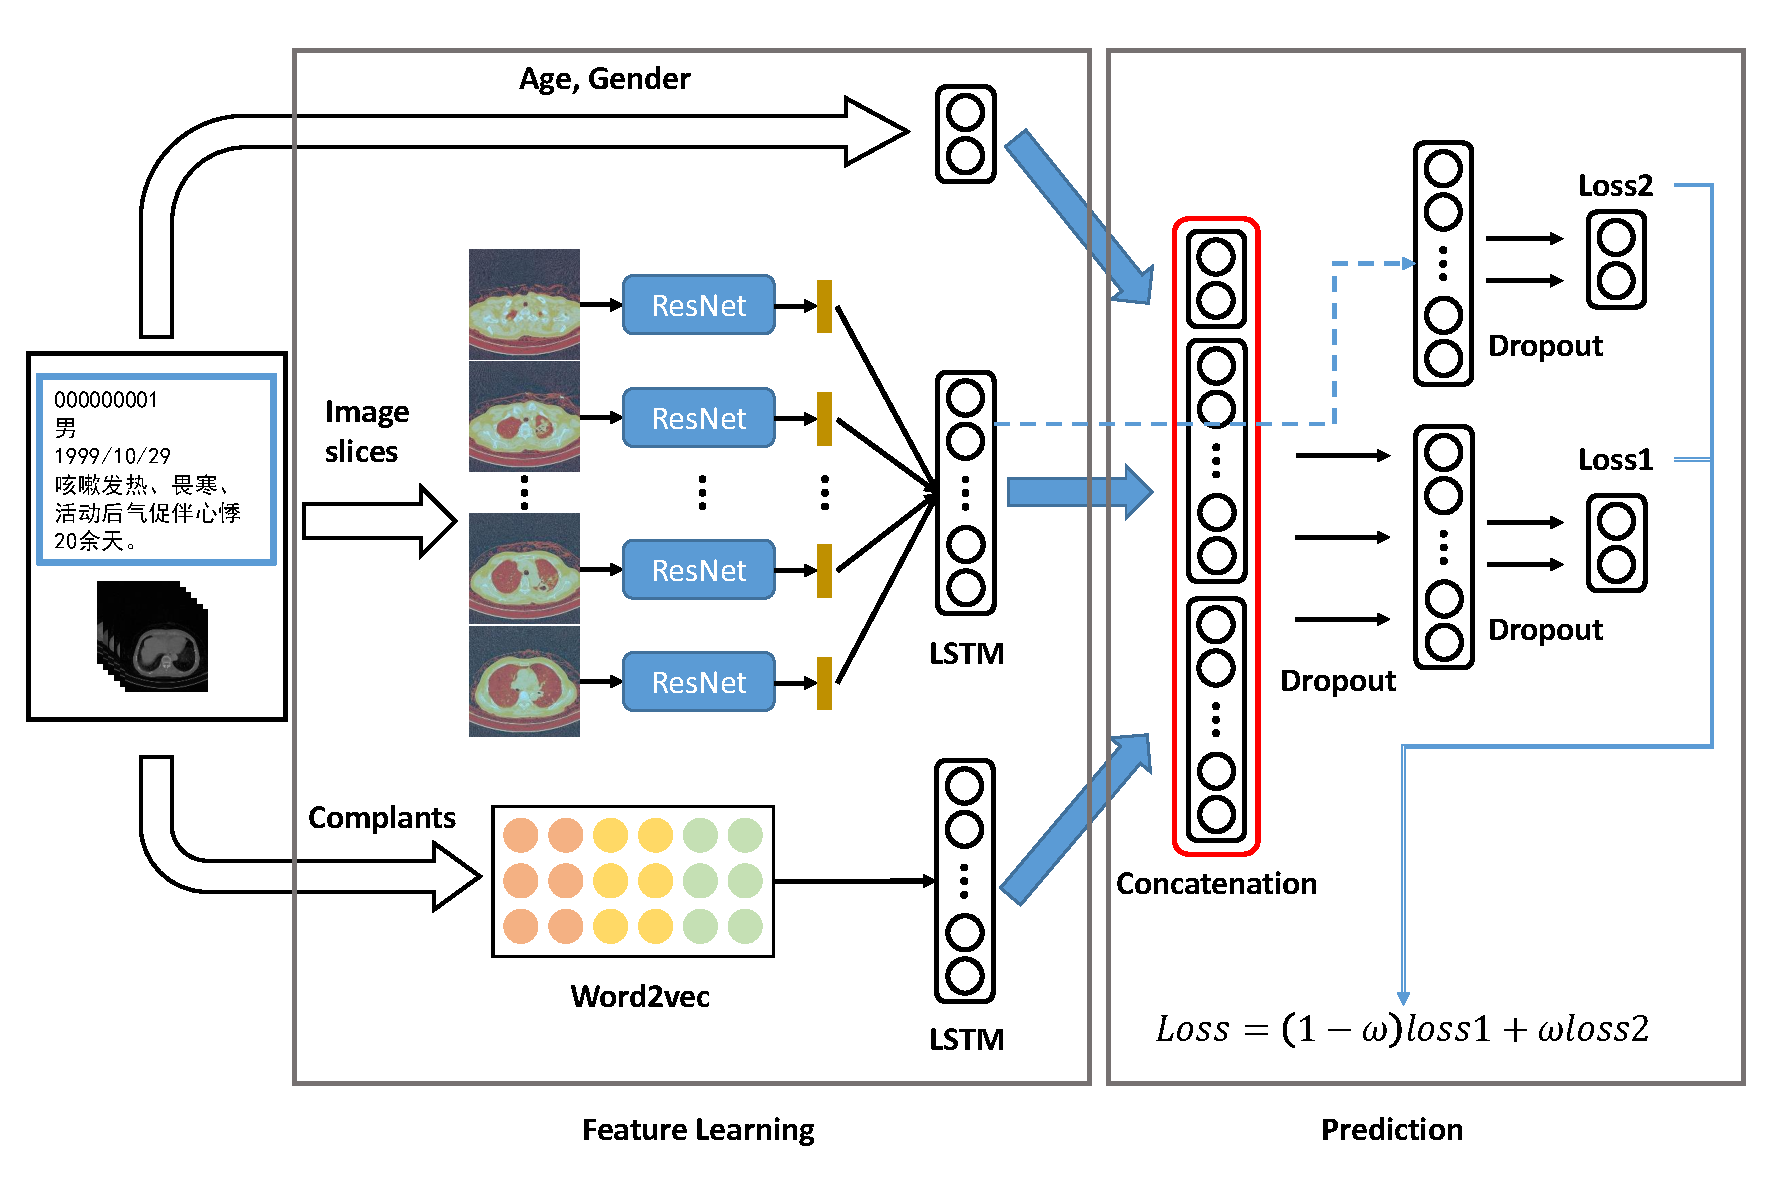
\includegraphics[width=130mm]{MSID.pdf}}
    \vspace{-0cm}
    \caption{Multi-Source Information Diagnosis Model}
    \vspace{-0cm}
    \label{msid}
    \end{figure}

\begin{table}[htb]
    \vspace{-0cm}
    \caption{Weights of Two Losses at Different Training Step}
    \vspace{-0cm}
    \begin{center}
    \begin{tabular}{|c|c|c|}
    \hline
    \textbf{\textit{Number of Steps}} & \textbf{\textit{$1 - \omega$}} & \textbf{\textit{$\omega$}}\\
    \hline
    602 &0.6238 & 0.3762  \\
    9030 &0.6547 & 0.3453  \\
    18060 &0.7027 & 0.2973  \\
    27090 &0.7185 & 0.2815  \\
    36120 &0.7234 & 0.2766  \\

    \hline
    \end{tabular}
    \vspace{-0cm}
    \label{weights}
    \end{center}
    \vspace{-0cm}
    \end{table}

\subsection{Training}
\label{training}
There two steps during training process.
The first step is to train difference kinds of RCNN to get the best structure, the outputs from RCNN($1 \times 256$) will be feed into two fully connected layers to get classification results, as shown in Fig~\ref{onestream}. We compare three kinds of classic CNN models: VGG16, GoogleNet with Inception-V3, ResNet50. VGG16 is relatively shallow, ResNet50 is deepest in these three kinds of models. We tried to use deeper network like ResNet101, however using ResNet101 make the training of model very slow and bring a heavy burden to servers. So we keep ResNet50 in RCNN.

The second step is to train MSID model. We use model get in the first step as feature extractor for images, use LSTM as feature extractor for complaints, and combine them with information of age and gender. All these features will be feed into two fully-connected layers to get final classification results.

Moreover, we use CNN models pre-trained on ImageNet\cite{ILSVRC15}. Models without pre-training is almost impossible to train because it won't converge or converge very slow during training. As Table~\ref{pretrain} shown, using pre-trained models can significantly improve the converging speed.

\begin{table}[htb]
    \vspace{-0cm}
    \caption{Comparison between training from scratch and training with pre-trained weights}
    \vspace{-0cm}
    \begin{center}
    \begin{tabular}{|c|c|c|c|c|c|c|}
    \hline
    \textbf{\textit{Structure}} & \textbf{\textit{Pre-trained}} & \textbf{\textit{Data}}& \textbf{\textit{Accuracy}}  & \textbf{\textit{Sensitivity}} & \textbf{\textit{Specificity}} & \textbf{\textit{AUC}}\\
    \hline
    ResNet50+LSTM &No & Normal & 0.545 & 1.0 &0.0 &0.57 \\
    GoogleNet+LSTM & No & Normal & 0.545 & 1.0 & 0.0 &0.5\\
    ResNet50+LSTM & Yes & Normal & 0.925 & 0.954 & 0.890 & 0.922\\
    GoogleNet+LSTM & Yes & Normal & 0.865 & 0.826 & 0.912 & 0.869\\
    
    \hline
    \end{tabular}
    \vspace{-0.5cm}
    \label{pretrain}
    \end{center}
    \vspace{-0.5cm}
    \end{table}

Initial learning rate is set 0.0005 and drops 50\% every 3000 training steps. The dropout rate in fully connected layers is set to 0.5, and dropout rate in LSTM is set to 0.3.

\section{Experiments and Results}
\label{exp}
In order to prove the effect of CNN, auxiliary loss and multi-source information, we run a lot of experiments to compare with each other, and the results of experiments is shown in Table~\ref{comparison}.

First of all, we do experiments to prove the effect of images with three ranges of HU values. We can see that RCNN(ResNet), RCNN(GoogleNet) and RCNN(VGG) trained by three channel image all have better performance than these models trained by one channel data. 
For RCNN(VGG), model trained by three channel image outperforms model train by Normal Image in accuracy,specificity and AUC score. Even if RCNN(VGG) with Normal Image has better performance in sensitivity, we can see that it only get 0.626 in specificity, which means this model is not been trained well. For RCNN(ResNet) and RCNN(GoogleNet), we can see that these two models trained by Three Channel Image perform best compared to models trained by Normal Image, High Attenuation Image and Low Attenuation Image. Especially RCNN(ResNet) trained by Three Channel Image, it get 0.93 in accuracy, 0.934 in specificity, 0.93 in AUC score, which are highest in six versions of experiments. RCNN(ResNet) trained by Normal Image has 0.954 in sensitivity, which is the highest in six experiments, but it only achieve 0.824 in specificity, which corrupts the performance of whole model. As a result, we use RCNN(ResNet) as our feature extractor for image information, and all images will be transformed into three ranges of HU values and compressed into three channel images.

Then we run a experiment to prove the effectiveness of auxiliary loss. We train RCNN(ResNet) with three channel image, but we set $\omega$ to $1$, which means we remove the gradient propagates directly to CNN and the model actually has only one loss. We can see that the performance of RCNN with single loss drops around 1\% in all four indication. It proves that, by using auxiliary loss, CNN will be trained in a better way. 

At last, we run experiments to prove than multi-source information can enhance the performance of CAD system. As shown in section~\ref{msid}, the ourput of RCNN($1 \times 256$), output of LSTM for complaints($1 \times 50$) gender($1 \times 1$) and age($1 \times 1$) will be concatenated together($1 \times 308$) and fused by two fully-connected layers, and build MSID. It is simple, but effective. We can see that MSID has the highest score in accuracy, specificity and AUC score. But it achieves 0.936 in sensitivity, 1.8\% lower than the highest 0.954. It means MSID has the best performance of classification according to its AUC score.

\begin{table}[htb]
    \vspace{-0cm}
    \caption{Comparison of All Kinds of RCNN and MSID}
    \vspace{-0cm}
    \begin{center}
    \resizebox{\textwidth}{23mm}{
    \begin{tabular}{|c|c|c|c|c|c|}
    \hline
    \textbf{\textit{Structure}} & \textbf{\textit{Data}}& \textbf{\textit{Accuracy}}  & \textbf{\textit{Sensitivity}} & \textbf{\textit{Specificity}} & \textbf{\textit{AUC}}\\
    \hline
    RCNN(VGG) & Normal Image & 0.805 & {\bfseries 0.954} &0.626 &0.790 \\
    RCNN(VGG) & Three Channel Image& 0.890 & 0.927 &0.846 &0.886 \\
    RCNN(GoogleNet) & Normal Image& 0.865 & 0.826 & 0.912 & 0.869 \\
    RCNN(GoogleNet) & High Attenuation Image& 0.880 & 0.853 & 0.912 & 0.883 \\
    RCNN(GoogleNet) & Low Attenuation Image& 0.860 & 0.890 & 0.824 & 0.857 \\
    RCNN(GoogleNet)& Three Channel Image & 0.905 & 0.900 & 0.912 & 0.906 \\
    RCNN(ResNet) & Normal Image & 0.925 & {\bfseries 0.954} & 0.890 & 0.922 \\
    RCNN(ResNet)& High Attenuation Image& 0.875 & 0.908 & 0.835 & 0.872 \\
    RCNN(ResNet) & Low Attenuation Image& 0.865 & 0.900 & 0.824 & 0.861 \\
    RCNN(ResNet), Single Loss & Three Channel Image& 0.920 & 0.917 & 0.923 & 0.920 \\
    RCNN(ResNet) & Three Channel Image& 0.930 & 0.927 & 0.934 & 0.930 \\
    MSID & Multi-Source Data&  {\bfseries 0.945} & 0.936 & {\bfseries 0.956} & { \bfseries 0.945} \\
    \hline
    \end{tabular}}
    \vspace{-0cm}
    \label{comparison}
    \end{center}
    \vspace{-0cm}
    \end{table}

The validation loss and accuracy during training is shown in Fig~\ref{aac} and Fig~\ref{loss}. We can see that In Fig~\ref{aac}, MSID can achieve higher accuracy at the first phase of training, but RCNN(ResNet), RCNN(GoogleNet) and RCNN(ResNet) with single loss perform better after. Until 27000 training step, MSID's performance outperforms other methods. It is not hard to understand this phenomenon. Because MSID considers patients' information about age, gender and complaints, it can achieve about 0.70 in accuracy at the first training phase. But other methods has less parameters to be optimized, so they converge more quickly than MISD. We can also see RCNN(ResNet), RCNN(ResNet) with single loss have similar performance during training, but RCNN(ResNet) wit auxiliary loss perform a little bit better than RCNN(ResNet) with single loss at the end of training. For RCNN(GoogleNet), it converge slower than RCNN(ResNet) and RCNN(ResNet) with single loss, and has a lower accuracy in the end.

The phenomenon shown in Fig~\ref{loss} is also can be explained. RCNN(GoogleNet) has the highest loss at the end of training, so it perform the worst in accuracy. RCNN(ResNet) and RCNN(ResNet) with single loss have the similar loss. MSID's loss decrease steadily, even if it has the highest loss for a moment during training, but it has the lowest loss after 27090 training steps.

\begin{figure}[htb]
    \centerline{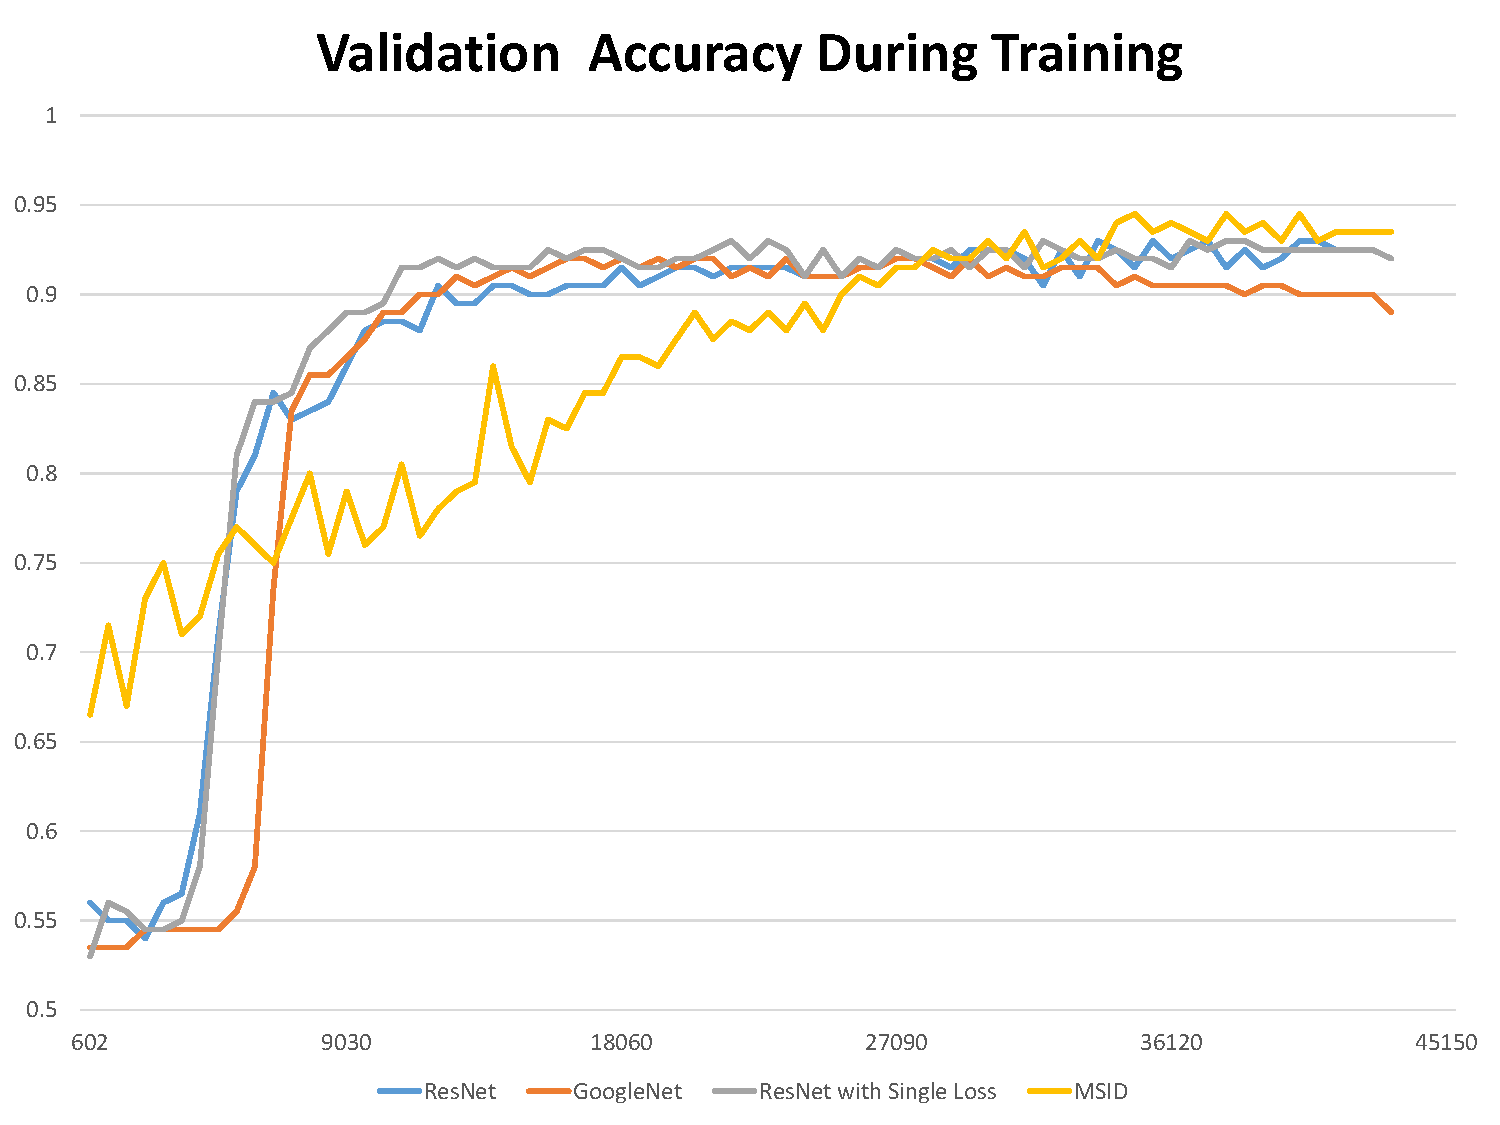
\includegraphics[width=100mm]{aac.pdf}}
    \vspace{-0cm}
    \caption{Validation Accuracy During Training}
    \vspace{-0cm}
    \label{aac}
    \end{figure}

\begin{figure}[htb]
    \centerline{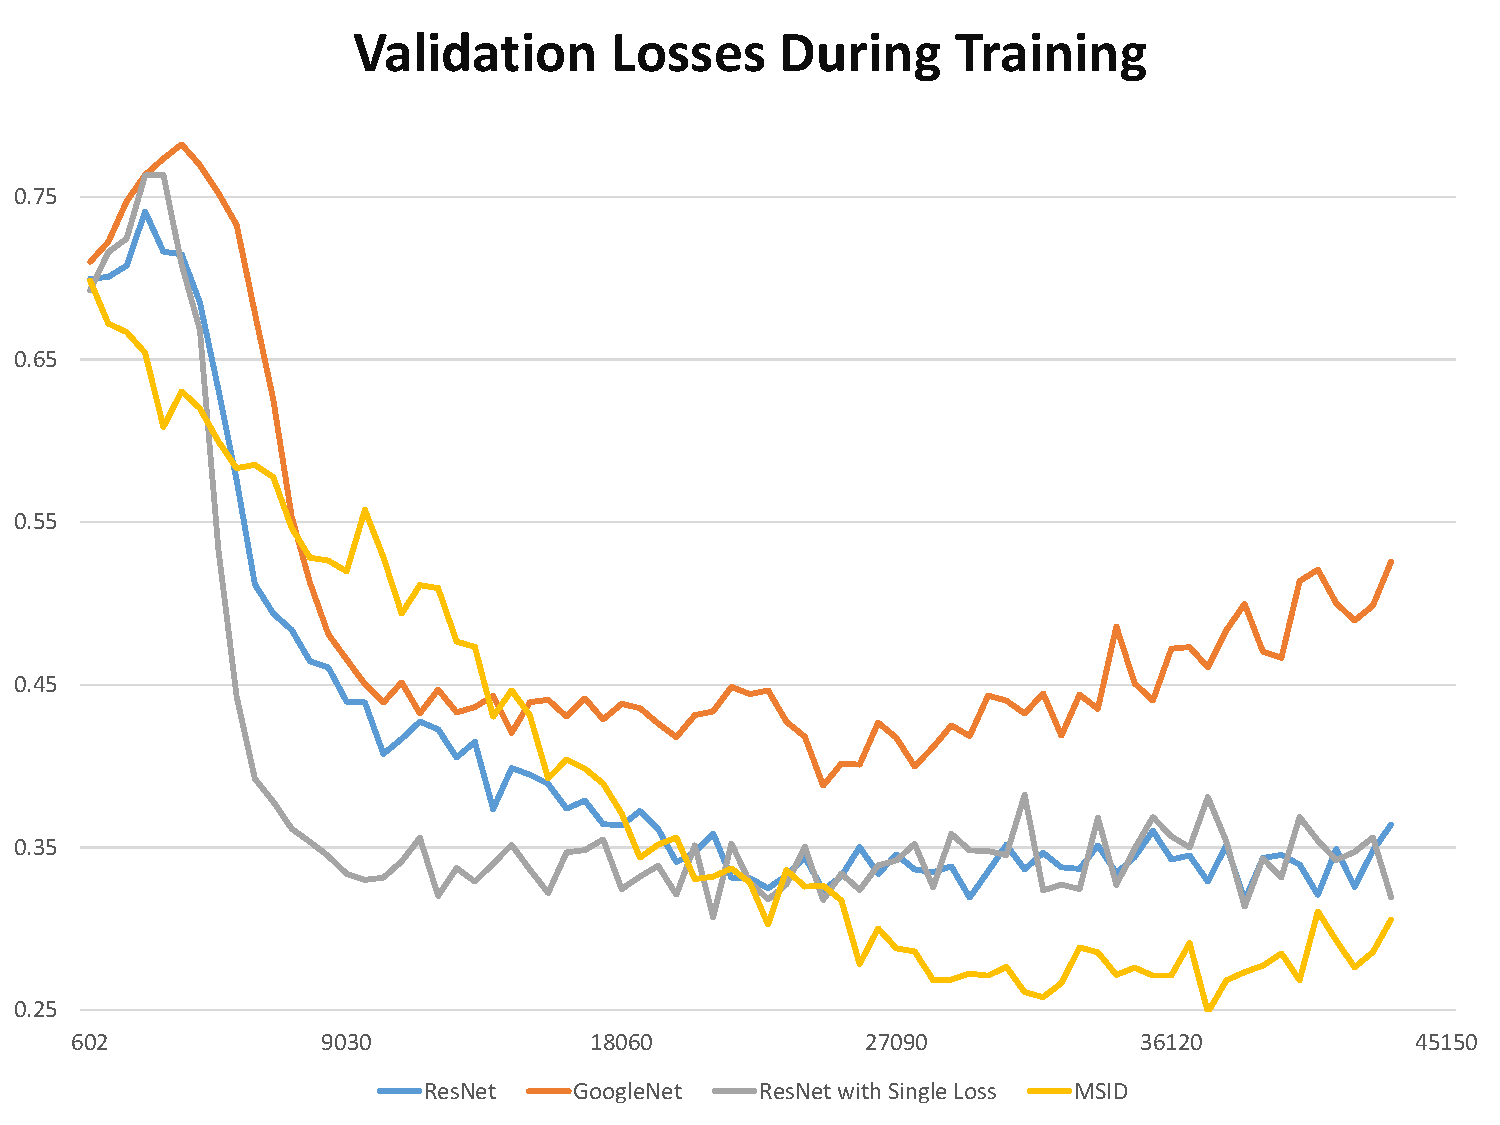
\includegraphics[width=100mm]{losses.pdf}}
    \vspace{-0cm}
    \caption{Validation Loss During Training}
    \vspace{-0cm}
    \label{loss}
    \end{figure}

\section{Conclusions}
\label{conclude}
In this study, we propose a novel model, MSID(Multi-Source Information Diagnosis), which combine CT image information with patients' age, gender and complaints. In MSID, CT scans will be treated like videos, and analysed by RCNN(Recurrent Convolutional Neural Network), complaints will be transformed into word vectors by word2vec and analysed by LSTM. Features from CT images and complaints will be fused together with patients' age and gender. All these information will be used to classify cases into healthy cases or pneumonic cases.

We analyze 1002 cases(450 healthy cases and 552 pneumonic cases). In fact, 1002 cases is far small than `big data', so our model's performance is restricted by data distribution and quality. However, in clinical practice, it is very difficult to construct a big scale medical dataset for deep learning, cause raw data is affected by radiologists' personal habits, data acquisition equipments, and hospital work rules. Our future work will focus on methods of data preprocessing which can over come difficulties mentioned above.
Moreover, our future work will also focus on fusing more source of information, like medical history, family history, blood test and other information witch will be considered during clinical practice. All works above will be carried out under the premise of respecting the privacy of the patients.
 

\bibliographystyle{unsrt}
\bibliography{refs}  

\end{document}
